
\chapter{Introduction}
\label{Chapter:introduction}

Dark Matter (DM) is one of the biggest mysteries in physics. There are various models that try to explain the abundance of DM in the universe, through extensions of the Standard Model (SM)\cite{Heeck_2015}\cite{vipandax}\cite{Dutra_2021}. The model we are focusing on has an ultralight pseudo-Nambu-Goldstone Boson (pNGB), as a DM candidate, which emerges from a Spontaneous Symmetry Breaking (SSB) \cite{Freitas_2021}.
In order to verify if the pNGB is a viable DM candidate we will do two analyses, first we will see if the pNGB will remain decoupled from the thermal bath, and second we will be using the misalignment mechanism, to calculate its relic density in the universe.

\section{History of Dark Matter}
In this section, we are going to talk about the historical evolution of DM, based on \cite{Bertone_2018}.
Perhaps the first person to talk about the existence of a specific unidentified astronomical object solely based on its gravitational influence was the mathematician Friederich Bessel.
In a letter that was published in 1844 \cite{1844bessel}, he made the following claim: 

\textit{If we were to think of Procyon and Sirius as double stars, their change in motion would not surprise us.} 

The motion of Sirius and Procyon could only be explained by the presence of faint companion stars that pull on the observed stars.

Lord Kelvin was one of the first to make an effort at a dynamical estimation of the Milky Way's dark matter abundance, he stated that the stars in the Milky Way can be thought of as gaseous particles moving under the force of gravity, and so we can determine the relation between the system's size and the star's velocity dispersion. 

The most well-known and frequently referenced pioneer in the study of dark matter was the Swiss-American astronomer Fritz Zwicky.
He discovered a significant scatter in the apparent velocities of eight galaxies inside the Coma Cluster in 1933, with differences exceeding 2000 km/s, but Zwicky went one step further and used the virial theorem to calculate the cluster's mass \cite{1933zwicky}.

He discovered that a sphere of $10^6$ light-years should contain 800 galaxies with a mass of $10^9$ solar masses and a velocity dispersion of \SI{80}{\km/\s}.
On the other hand, the average velocity dispersion along the line of sight was observed to be around \SI{1000}{\km/\s}.

\textit{If this would be confirmed, we would get the surprising result that dark matter is present in a much greater amount than luminous matter}

Assuming galaxies are in virial equilibrium, one would expect, $M(r) \propto v^2r/G$, and  be able to connect the mass of a galaxy at a given distance $r$ from the galaxy's center.

\begin{figure}[H]
	\centering
	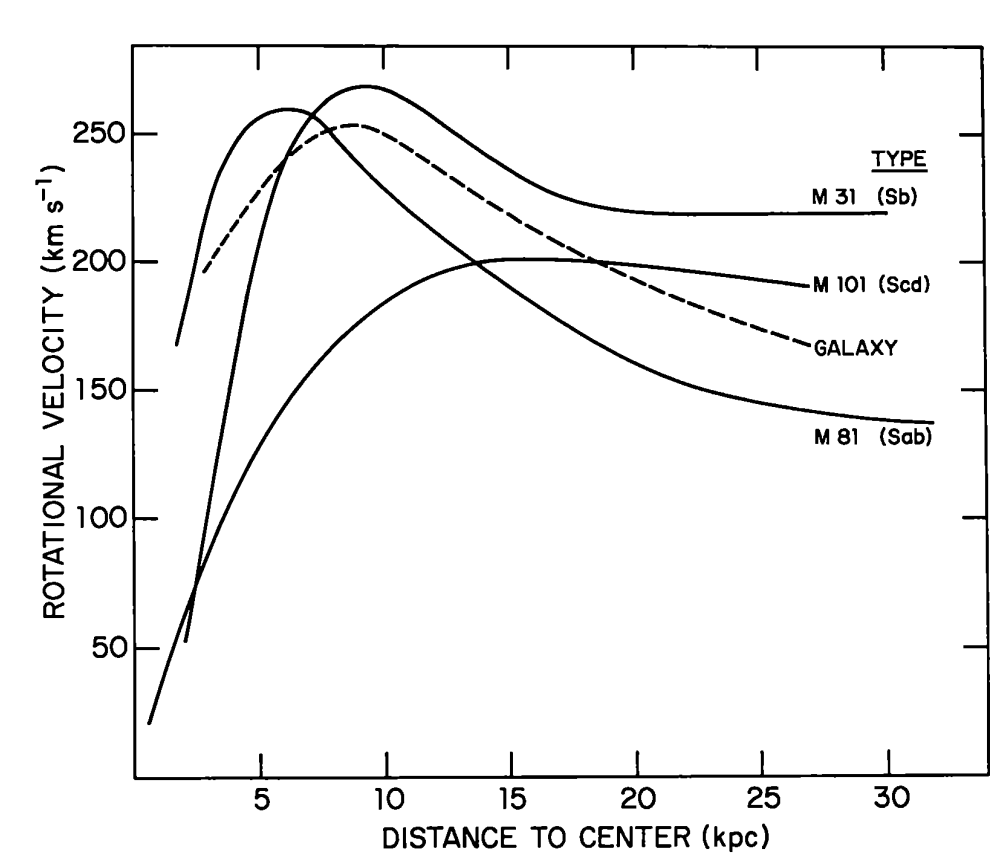
\includegraphics[width=0.6\linewidth]{graphs/rotation-curves}
	\caption{Rotation curves of various galaxies \cite{1973rotationcurves}, where the continuous lines represents the rotational velocity measured experimentally and the dashed one  represents the theoretical prediction.}
	\label{fig:rotation}
\end{figure}

As shown in \autoref{fig:rotation}, this is not the case, as $v$ is constant outside the galaxy's center, which indicates that $M \propto r$ outside the center.
This is one of the most compelling arguments for the existence of dark matter. 

\section{Dark Matter as a particle}

The term "dark matter"\ itself has undergone significant change during the previous few decades.
Today, this phrase is most usually used to refer to the particles that make up the majority of the matter density in our universe. Via the Cosmic Microwave Background (CMD), we can say that the current matter density of the universe is, $\Omega^0h^2\simeq0.13$, and the current baryonic matter density of the universe is, $\Omega^0h^2\simeq0.0225\pm0.00023$, baryonic matter is matter that makes up protons and neutrons \cite{2020}. By a simple subtraction we can calculate the non-baryonic matter density to be, $\Omega^0h^2\simeq0.11$, which allows us to see that most of the matter that makes up the universe aren't particles that constitute atoms, this non-baryonic matter is DM.

DM can be produced through: Freeze-in, Freeze-out, cosmic strings, domain walls and misalignment \cite{kolb}\cite{Marsh_2016}\cite{GONDOLO}\cite{Hall:2009bx}.

When looking at the DM problem through the perspective of the SM of particle physics, the three neutrinos stand out, as we notice that DM has characteristics very similar to neutrinos. The main properties of DM are its stability, neutrality, it only interacts with gravitational fields, and its cold, after the structure formation.
In contrast to every other known particle types, neutrinos are stable - or at least very long lived - and do not interact with electromagnetic or strong fields. These are some of the necessary properties for practically any viable candidate for dark matter\cite{STEIGMAN1985375}.
And even though we now know that dark matter in the form of neutrinos from the standard model would not be able to explain the observed large-scale structure of our Universe, these particles serve as a crucial model for an hypothetical class of particles, known as WIMPs, or weakly interacting massive particles. 
In this day and age, WIMPs are the strongest candidate for DM, but the lack of experimental evidence makes physicists lose interest in this candidate \cite{Moore_1999}\cite{10.1093/mnras/193.2.189}.

The main property of a given dark matter candidate, that numerical simulations can examine is whether it was relativistic (hot) or non-relativistic (cold) during the period of structure formation ($T\sim 10^5K$).

Lately, there has been a lot of interest focused on ultralight particles for DM candidates, with masses around $m\sim\mathcal{O}\left(10^{-10}-10^{-20}\right)\si{\eV}$,  
however these particles cannot be detected through direct detection experiments, but there have been developments in the area of gravitational waves that can uncover the truth about this hypothesis, which will be the main topic in this work.